\begin{center}
\large\noindent\fbox{
	\parbox{\textwidth}{
Con riferimento al sistema lineare dell' Esercizio 6.3, con $n=1000$, graficare la norma dei residui, rispetto all'indice di iterazione, generati dai metodi di Jacobi e Gauss-Seidel. Utilizzare il formato \textit{semilogy} per realizzare il grafico, corredandolo di opportune $label$.
} }
\end{center}

\noindent Il seguente codice Matlab \'e stato utilizzato per la risoluzione del problema:

\lstinputlisting[language=Matlab]{Codici/Cap6/SoluzioneEs5_Cap6.m}

\vspace*{1cm}

\noindent Il grafico seguente mostra la norma dei residui, rispetto all'indice di iterazione generati dai metodi di Jacobi (in azzurro) e Gauss-Seidel (in rosso):


\begin{figure}[H]
	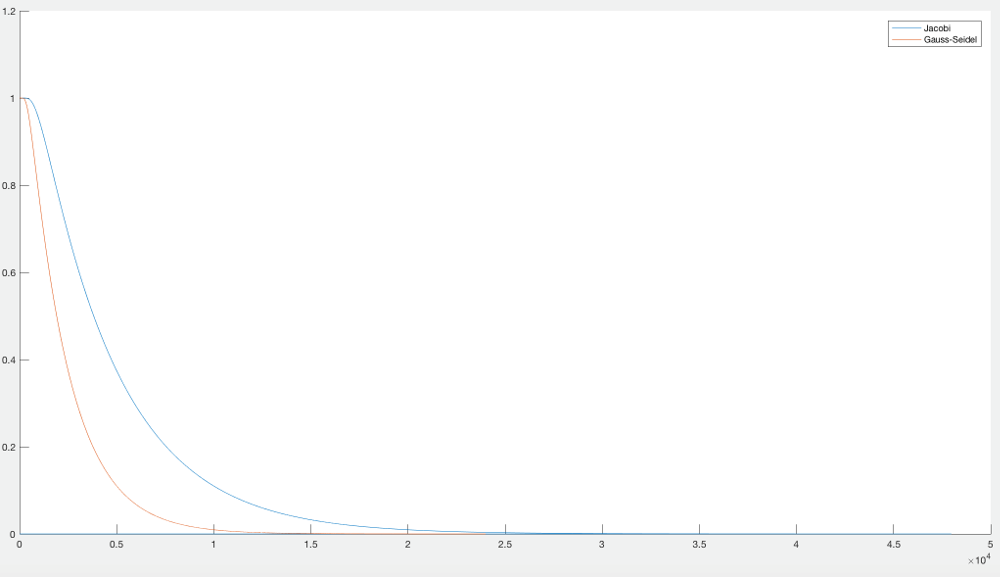
\includegraphics[width=\textwidth]{Codici/Cap6/Es5_Cap61}
\end{figure}